\section{Maps \& Hash Tables}
\scriptsize{hash function}\\ 
{\tiny a one-way function that takes a variable-length object and turns it into a fixed-length bit string\\
most common application: set, map (associative array/dictionary/symbol table)\\
other applic.: database indexing, cache management, efficient duplicate detection, file signature verification against corrupt/tempered files, password storage, electronic signatures, part of many cryptographic algorithms/applications
}\\
\scriptsize{set}\\ {\tiny abstract data type, unordered collection without duplicates\\
basic operations: x in s, s.add(x), s.remove(x)
}\\
\scriptsize{map}\\ {\tiny abstract data type, a collection that allows indexing with almost any data type (Python dict require immutable data type)\\
basic operations: d[key], d[key]=val, del d[key]
}\\
{\tiny implement sets and maps:\\}
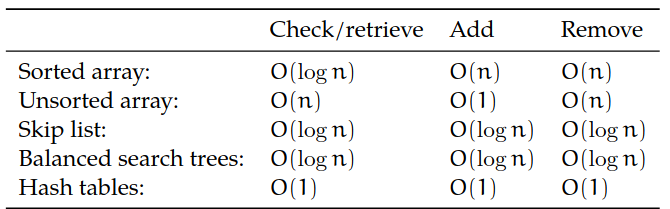
\includegraphics[scale=0.15]{sets_maps.png}\\
\scriptsize{hash function}\\
{\tiny h() maps a key to an integer index between 0 and m(size of array)\\
we use h(k) as an index to an array(of size m)\\
collision: occurs if 2 different key values are mapped to the same integer\\
2 parts: map any object (variable bit string) to an integer (e.g., 32 or 64 bit); compress the range of integers to map size(m)\\
main challenge with implementing hash maps: avoid and handle the collisions
}\\
\scriptsize{compress hash codes}\\ 
{\tiny easy way: use modulo m+1 to map any integer to range [0,m]\\
good hash functions minimize collisions, but collisions occur\\
2 common approaches to handle collisions: separate chaining, open addressing
}\\
\scriptsize{separate chaining} {\tiny each array element keeps a pointer to a secondary container(typically a list); when an collision occurs, add the item to the list\\
complexity: all operations require locating the element first, cost include hashing(constant)+search in secondary data structure, worst-case O(n)\\
with a good hash function, the probability of collision is n/m, O(n/m)=O(1) (if m>n)\\
expected complexity for all operations is O(1)
}\\
\scriptsize{load factor} {\tiny = num of entries/num of indices\\
low load factor: better run time (fewer collisions)/more memory usage\\
when load factor is over a threshold, the map is extended(needs rehash)\\
around 0.75 is considered optimal
}\\
\scriptsize{open addressing(linear probing)} {\tiny during insertion, if there is a collision, look for the next empty slot and insert\\
during lookup, probe until there is an empty slot\\
when delete an element, insert a special value that is treated as full during lookup and empty during insertion\\
tends to create clusters of items, especially if load factor is high(>0.5)\\
quadratic probing provides some improvement
}\\
\scriptsize{quadratic probing} {\tiny prob (h(k)+i**2) mod m for i=0,1,... until an empty slot is found\\
if m is prime and load factor is less than 0.5, guaranteed to find an empty slot\\
although better than linear probing, creates its own kind of clustering
}\\
\scriptsize{double hashing} {\tiny prob (h(k)+i*h'(k)) mod m for i=0,1,..., where h'(k) is another hash function\\
common choice: h'(k)=q-(k mod q) for a prime number q<m
}\\
\scriptsize{pseudo random number generator}
{\tiny prob $(h(k)+i*r_i) mod m$ for i=0,1,..., where $r_i$ is the i-th number generated by a peudo number generator\\
pseudo random number generators generate numbers that are close to uniform, given the same seed, the sequence is deterministic\\
the most common choice for modern programming languages, avoids problems with inputs that intentionally generate hash collisions
}\\
\scriptsize{has DoS attachs}\\ {\tiny a denial-of-service(DoS) attach aims to break or slow down an internet site/service\\
input to a web-based program is passed as key-value pairs, which are typically stored in a dictionary\\
if one intentionally posts an input with large number of colliding keys, the hash table implementation needs to chain long sequences or probe large number of times and eventually re-hash\\
this increases expected to O(1) time to worst-case complexity
}\\
\scriptsize{xor or add}\\
{\tiny hash codes must be consistent: if a==b, h(a)==h(b)\\
should minimize collisions, values for h should be uniformly distributed\\
should be fast to compute (or not if used for passwords\\
simple appraoch: bitwise add (or XOR) each k-bit segment of the memory representation of the object, ignoring the overflow\\
in practice create many collisions due to associativity (abc, bca and cba get the same hash code)
}\\
\scriptsize{polynomial hash codes}\\
{\tiny multiply with powers of a constant, will produce different values with sequences with the same items in different order\\
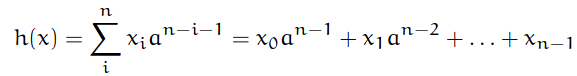
\includegraphics[scale=0.2]{poly_hash.png}
}\\
\scriptsize{cyclic-shift hash codes}\\
{\tiny shifts some bits from one end to the other at each step in the running sum\\
a fast way of obtaining a non-associative valid hash code since bitwise operations are simple \\
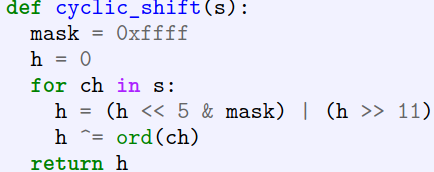
\includegraphics[scale=0.2]{cyclic_shift.png}
}\\
\scriptsize{cryptographic hash functions} {\tiny in cryptography, it is important to have hash functions for which it is difficult to find two keys with the same hash value\\
well-known hash functions: MD5, SHA-1, RIPEMD-160, Whirlpool, SHA-2, SHA-3, BLACK2, BLACK3\\
designed for applications like digital fingerprinting, password storage\\
computationally inefficient for use in data structures
}